\section{Atoms}
 
 The focus regarding atoms has been on simulating heavy atoms using a simple ansatz for the trial wave function, and thus test its limits. Due to the important nature of atoms in nature, precise experimental data which can be used to benchmark the results exist. Due to having an non-negligible relativistic nature, atoms which are heavier than Krypton are not simulated. The specifics regarding the model used for atoms are covered in Section \ref{sec:modelAtoms}.
 
\subsection{Ground State Energies}
 
 Table \ref{tab:AtomsRes} presents the ground state energy results for different atoms together with the experimental results. As expected, the helium ground state has the highest overlap with the corresponding experimental result. The relative precision of the heavier atoms are in the range $10^{-3}$ - $10^{-4}$, indicating that DMC performs equally well in all cases. However, the error in the calculations increase as the atoms become heavier. The calculations were done on a single node; running the calculations on several nodes with an increased number of walkers could reduce the error somewhat. 
 
 As expected, VMC performs rather poorly compared to DMC. In comparison to quantum dots, where the two methods produced significantly similar energies, atoms have an addition approximation in the trial wave function due to the fact that the solid harmonics are used instead of the spherical harmonics. This is covered in detail in Section \ref{sec:modelAtoms}. This fact further demonstrates that DMC, unlike VMC, has the power to perform well even in situations where the trial wave function is not optimal. 
 
\begin{table}
\begin{center}
\begin{tabular}{lp{2cm}cclc}
Atom & & $E_\mathrm{VMC}$ & \qquad $E_\mathrm{DMC}$ & \qquad\,\, Expt. & \qquad $\epsilon_\mathrm{rel}$\\
\hline\hline
\ \\
He & \qquad & -2.8903(2) & \qquad -2.9036(2) & \qquad $-2.9037$ & \qquad $3.44\cdot 10^{-5}$\\
\ \\
Be & \qquad & -14.145(2) & \qquad -14.657(2)  & \qquad $-14.6674$ & \qquad $7.10\cdot 10^{-4}$ \\
\ \\
Ne & \qquad & -127.853(2) & \qquad -128.765(4) & \qquad $-128.9383$ & \qquad $1.34\cdot 10^{-3}$  \\
\ \\
Mg & \qquad & -197.269(3) & \qquad -199.904(8) & \qquad $-200.054$ & \qquad $7.50\cdot 10^{-4}$  \\
\ \\
Ar & \qquad & -524.16(7) & \qquad -527.30(4) & \qquad $-527.544$ & \qquad $4.63\cdot 10^{-4}$  \\
\ \\
Kr & \qquad & -2700(5) & \qquad -2749.9(2) & \qquad $-2752.054976*$ & \qquad $7.83\cdot 10^{-4}$  \\
\ \\
\end{tabular}
\caption{Ground state energies for Atoms calculated using Variational - and Diffusion Monte-Carlo. Experimental energies are listed in the last column. As we see, DMC is rather close to the experimental energy. $\epsilon_\mathrm{rel} = |E_\mathrm{DMC} - \mathrm{Expt.}|/|\mathrm{Expt.}|$. Experimental, i.e. ``exact'' energies are taken from Ref. \cite{AtomsExact} for He through Ar, and \cite{KryptonExact} for Kr. (*) The referenced Krypton result is not a direct experimental result, but obtained by Hartree-Fock calulcations with optimized single particle wave functions, and is thus believed to be a very good approximation to the exact ground state.}
\label{tab:AtomsRes}
\end{center}
\end{table}
 
 
 \subsection{One-body densities}
 
 The one-body densities for the \textit{noble gases}, that is, the closed shell atoms, are presented in Figure \ref{fig:OBD_noble_Atoms_2D_combo}. Comparing these to the one-body densities for the alkaline earth metals, i.e. $\mathrm{Be}$, $\mathrm{Mg}$, etc., in Figure \ref{fig:OBD_alkaline_Atoms_2D_combo}, it is clear that the noble gases have a more confined electron distribution. This corresponds well to the fact that noble gases do not form compound materials, i.e. molecules \cite{UniversityPhysics}. The alkaline earth metals on the other hand are found naturally as parts of compound materials. The one-body densities of the alkaline earth metals spreading out in space are thus in excellent agreement with nature.
 
 The attractive nature of the nuclear potential is demonstrated by the core having an extremely high electron density, independent of the number of electrons. The radial density is thus not very insightful, however, multiplied with the radius squared, the difference between atoms become noticeable.
 
It is apparent that the VMC distribution and the pure distribution differ more in the case of alkaline earth metals than for noble gases. This implies that the trial wave function is better in the case of noble gases. To explain this phenomenon, it is important to realize that for closed shell systems, there is only one configuration with the lowest possible non-interacting energy. For open shell systems, there are several ways of configuring the electrons which produce the same non-interacting energy. This is due to the fact that the single particle energy is independent of the angular and azimuthal quantum numbers $l$ and $m$ introduced in Section \ref{sec:modelAtoms}.

For instance, Beryllium has two electrons in the $n=1$ state and two in the $n=2$ state. The trial wave function used in this thesis uses the $m=l=0$ states only for beryllium, however, in light of the previous paragraph, the wave function suffers from the fact that the $l=1$ states are equally energy efficient. In order to have an equally optimal ansatz in the case of alkaline earth metals as in the case of noble gases, the contributions from these equally efficient states must be included. 
 
 
 
 \begin{figure}
 \begin{center}
   \subfigure{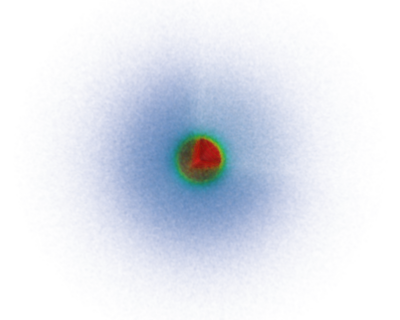
\includegraphics[scale=0.4]{../Graphics/OBD/OBD_Atoms/3D/Beryllium.png}} 
   \subfigure{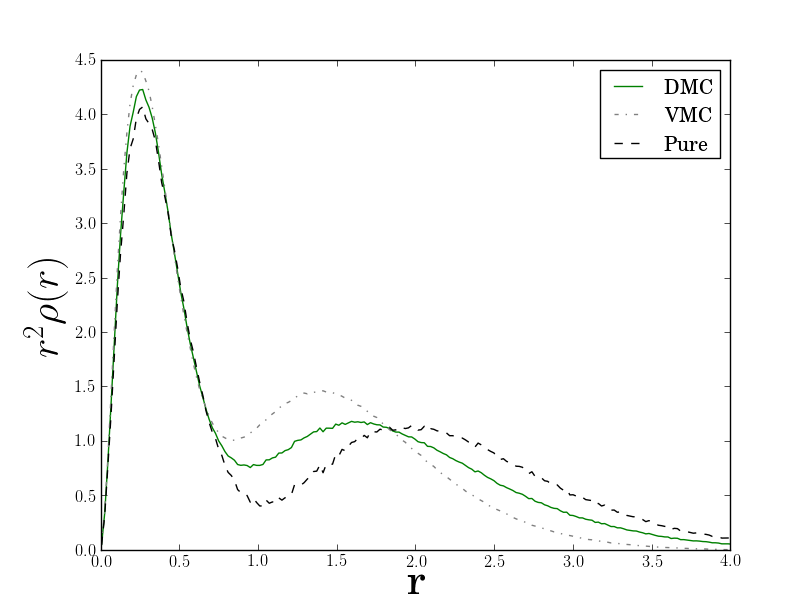
\includegraphics[scale=0.3]{../Graphics/OBD/OBD_Atoms/2D/Beryllium.png}}  \\
   \subfigure{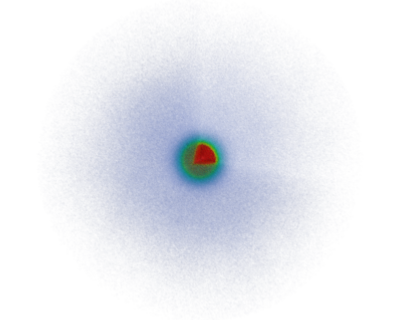
\includegraphics[scale=0.4]{../Graphics/OBD/OBD_Atoms/3D/Magnesium.png}} 
   \subfigure{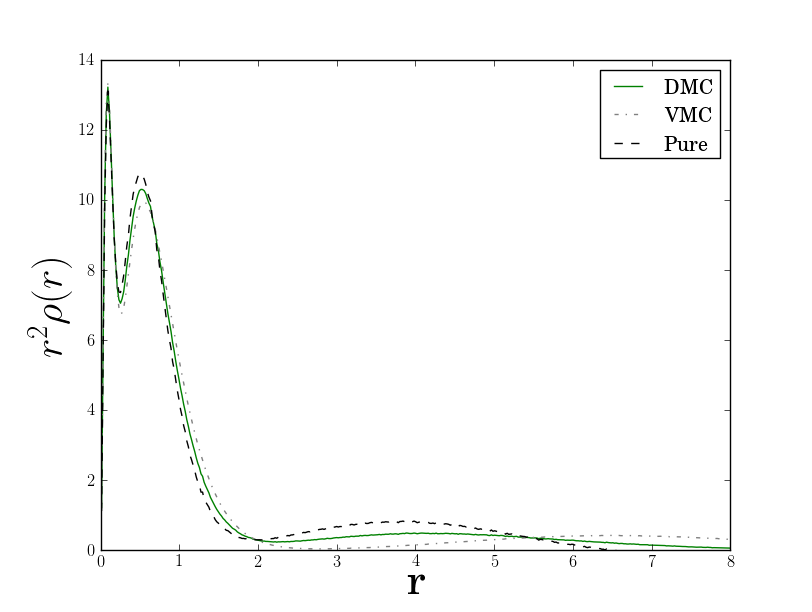
\includegraphics[scale=0.3]{../Graphics/OBD/OBD_Atoms/2D/Magnesium.png}}  \\
  \caption{Three dimensional one-body density (left column) and angular averaged radii (right column) for alkaline earth metals; Beryllium (top) and Magnesium (bottom). The color bar shows increasing values from left to right. Notice that it is not the radial one-body density (which is too steep to reveal characteristics) in the right column, but the electron . Compared to the noble gases in Figure \ref{fig:OBD_noble_Atoms_2D_combo}, the alkaline earth metals have a surrounding dispersed probability cloud due to the broken closed shell symmetry. The element is thus more unstable and potent for chemical reactions and molecular formations through covalent - and ionic bonds \cite{UniversityPhysics}. Red and blue color implies a low and high electron density respectively.}
  \label{fig:OBD_alkaline_Atoms_2D_combo}
 \end{center}
\end{figure}
 
\begin{figure}
 \begin{center}
   \subfigure{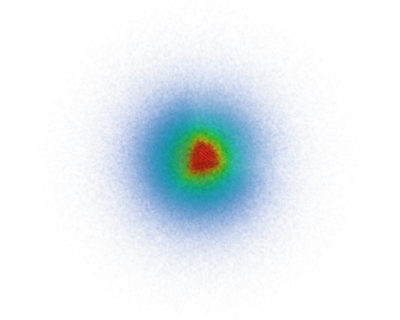
\includegraphics[scale=0.4]{../Graphics/OBD/OBD_Atoms/3D/Helium.png}} 
   \subfigure{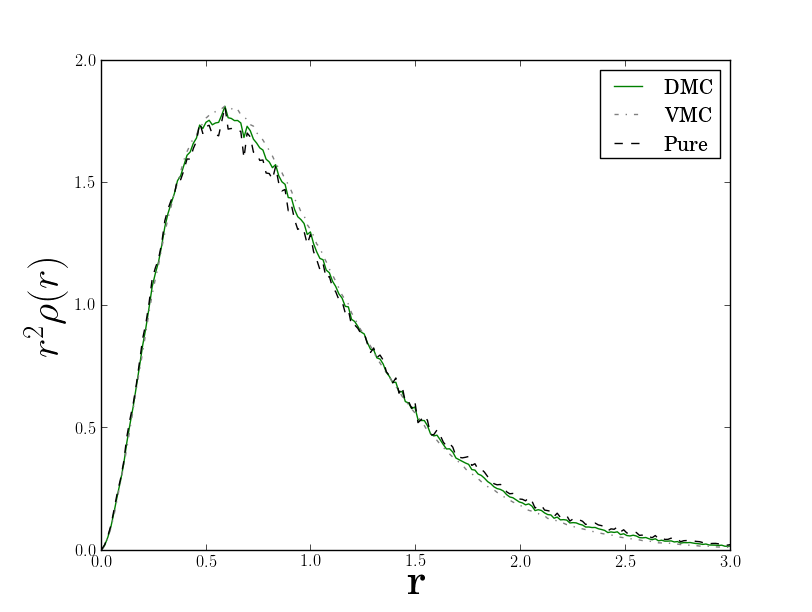
\includegraphics[scale=0.3]{../Graphics/OBD/OBD_Atoms/2D/Helium.png}}  \\
   \subfigure{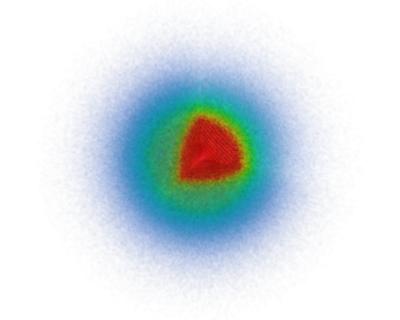
\includegraphics[scale=0.4]{../Graphics/OBD/OBD_Atoms/3D/Neon.png}} 
   \subfigure{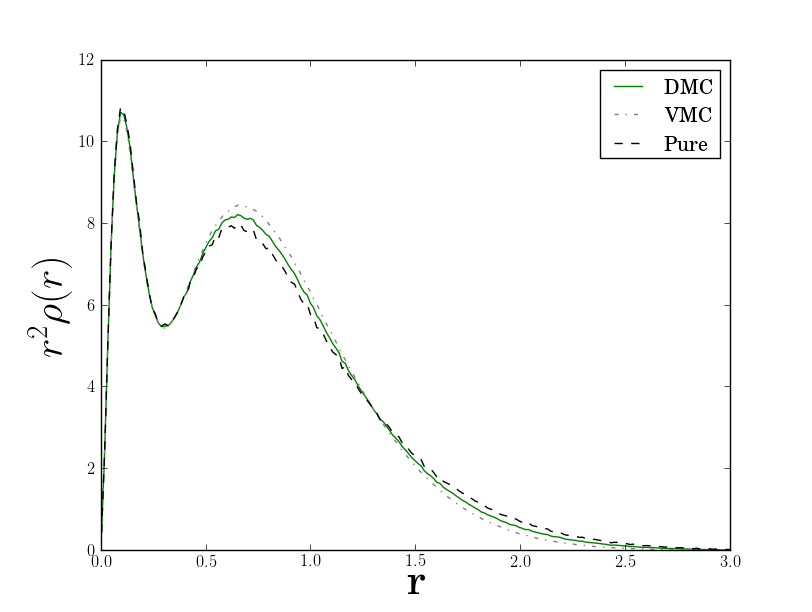
\includegraphics[scale=0.3]{../Graphics/OBD/OBD_Atoms/2D/Neon.png}}  \\
   \subfigure{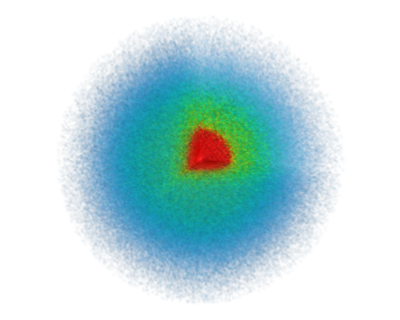
\includegraphics[scale=0.4]{../Graphics/OBD/OBD_Atoms/3D/Argon.png}} 
   \subfigure{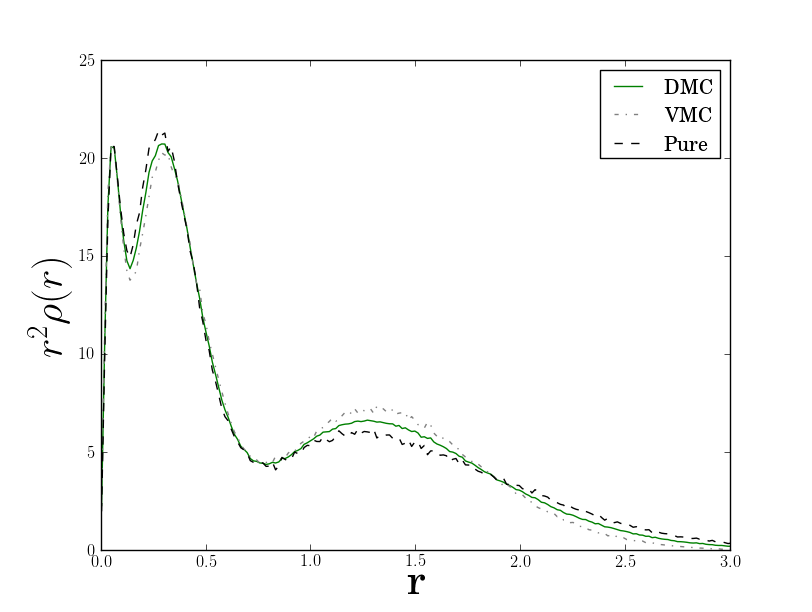
\includegraphics[scale=0.3]{../Graphics/OBD/OBD_Atoms/2D/Argon.png}}  \\
   \subfigure{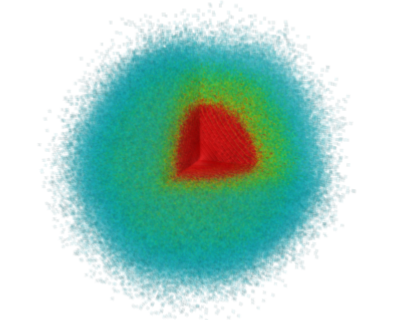
\includegraphics[scale=0.4]{../Graphics/OBD/OBD_Atoms/3D/Krypton.png}} 
   \subfigure{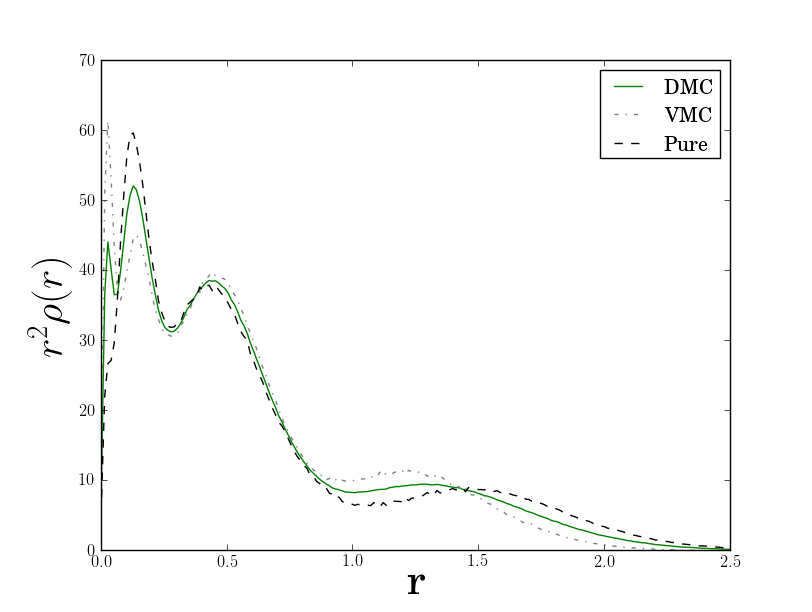
\includegraphics[scale=0.3]{../Graphics/OBD/OBD_Atoms/2D/Krypton.png}}  \\
  \caption{One-body densities for noble gases. Counting top to bottom: Helium, Neon, Argon and Krypton. A quarter of the spherical density is removed to present a better view of the core. Red and blue color implies a low and high electron density respectively.}
  \label{fig:OBD_noble_Atoms_2D_combo}
 \end{center}
\end{figure}
 
 
